% Thesis paper
% submitting to RV 2015
% spring 2015
% Aaron Kane

%\documentclass[]{Z:/Private/research/TeX/llncs/llncs}
\documentclass[]{llncs}
\pdfmapfile{+ltlfonts.map}

%\documentclass[]{C:/Users/akane/Documents/Research/TeX/llncs/llncs}
%% loading some packages, deleted all the info text from the ieee example page
\usepackage[nocompress]{cite}
\usepackage[cmex10]{amsmath}
\usepackage{amssymb}
\usepackage{url}
\usepackage{multirow}
% restore ieee style page breaks over multiline equations
%\interdisplaylinepenalty=2500
\usepackage{array}
\usepackage[table]{xcolor}
\usepackage[font=footnotesize,caption=false]{subfig}	% subfigures
%\usepackage{fixltx2e} 		% fixes ordering of single/double column figures
%% a couple packages we might want, but don't want to load yet
%\usepackage{algorithmic}
%\usepackage{eqparbox}
%\usepackage{syntax-mdw}
\usepackage{listings}
%\usepackage[pdftex]{graphicx}
\usepackage{graphicx}
%\graphicspath{{../pdf/}{../jpeg/}}
%\DeclareGraphicsExtensions{.pdf,.jpeg,.png}


%\addtolength{\textfloatsep}{-3.5cm}
%\addtolength{\floatsep}{-5cm}
\addtolength{\intextsep}{-5pt}
\addtolength{\belowcaptionskip}{-21pt}
%\usepackage{setspace}
%\doublespace
\usepackage{algorithmic}
%%% Omar based packages
\usepackage{ltlfonts}
\usepackage{mathtools}
\usepackage{xspace}


% proof/theorem stuff
%\newtheorem{thm}{Theorem}
%\newtheorem{tdef}{Definition}
%\newtheorem{lemma}{Lemma}
%\newtheorem{case}{Case}

% defines
\newcommand{\rp}[2]{\ensuremath{\langle #1, #2 \rangle}}
\newcommand{\res}[2]{\ensuremath{r_{#1}^{#2}}}
\newcommand{\agmon}{\ensuremath{\mathbf{agmon}}}
\newcommand{\precis}{\textit{pr\`ecis}\xspace}
\newcommand{\pst}{\ensuremath{S^i_\psi}}
\newcommand{\rpt}[3]{\ensuremath{\langle #1, #2 \rangle}_{#3}}
\newcommand{\greduce}{\textit{reduce}\xspace}
\newcommand{\nextmtl}{\bigcirc}
\newcommand{\lastmtl}{\dot\circ}

%%%%%%%%%%%%%% end preamble, begin doc %%%%%%%%%%%%%%%%%%%%%%%%%%%%%%%%%
\begin{document}

% paper title
% can use linebreaks \\ within to get better formatting as desired
%\title{Runtime Monitoring for Safety-Critical Embedded Systems: A Case Study}
\title{A Case Study on Runtime Monitoring of an Autonomous Research Vehicle (ARV) System}


\author{Aaron Kane\inst{1} \and Omar Chowdhury\inst{2} \and Anupam Datta\inst{1} \and Philip Koopman\inst{1}}
\institute{Carnegie Mellon University, Pittsburgh, PA
			\and  Purdue University, IN\\
			\email{akane@cmu.edu, ochowdhu@purdue.edu, danupam@cmu.edu, koopman@cmu.edu}}



% make the title area
\maketitle

%% comments
%\newcommand{\notes}[1]{}
\newcommand{\notes}[1]{\textcolor{red}{#1}}
\newcommand{\dg}[1]{\notes{Deepak says: #1}}
\newcommand{\limin}[1]{\notes{Limin says: #1}}
\newcommand{\anupam}[1]{\notes{Anupam says: #1}}
\newcommand{\omar}[1]{\notes{Omar says: #1}}

\newcommand{\eat}[1]{}
% \newcommand{\Paragraph}[1]{\vspace{5pt}\noindent\textbf{#1}}
\newcommand{\Paragraph}[1]{\vspace{2pt}\noindent\textbf{\textit{#1}}}
\newcommand{\evalPoint}{\ensuremath{\mathit{evalPtr}}\xspace}
\newcommand{\curPoint}{\ensuremath{\mathit{curPtr}}\xspace}

\newcommand{\etal}{\textit{et al.}\xspace}
\newcommand{\ie}{\textit{i.e.}\xspace}
\newcommand{\eg}{\textit{e.g.}\xspace}
\newcommand{\viz}{\textit{viz.}\xspace}
\newcommand{\etc}{\textit{etc.}\xspace}

\newcommand{\state}{\ensuremath{\pi}\xspace}
\newcommand{\statedown}[1]{\ensuremath{\pi_{#1}}\xspace}
\newcommand{\stateup}[1]{\ensuremath{\pi^{#1}}\xspace}
\newcommand{\structure}[1]{\ensuremath{\mathbb{S}_{#1}}\xspace}
\newcommand{\structureud}[2]{\ensuremath{\mathbb{S}_{#1}^{#2}}\xspace}
\newcommand{\idx}{\ensuremath{idx}\xspace}
\newcommand{\map}{\ensuremath{\mathcal{A}}\xspace}
\newcommand{\result}{\ensuremath{\mathbb{R}}\xspace}


\newcommand{\yesterday}{\ensuremath{\LTLcircleminus}\xspace}
\newcommand{\tomorrow}{\ensuremath{\LTLcircle}\xspace}
\newcommand{\henceforth}{\ensuremath{\LTLsquare}\xspace}
\newcommand{\eventually}{\ensuremath{\LTLdiamond}\xspace}
\newcommand{\historically}{\ensuremath{\LTLsquareminus}\xspace}
\newcommand{\once}{\ensuremath{\LTLdiamondminus}\xspace}
\newcommand{\since}{\ensuremath{\,\mathrm{\cal S}\,}\xspace}
\newcommand{\until}{\ensuremath{\,\mathrm{\cal U}\,}\xspace}
\newcommand{\weaksince}{\ensuremath{\,\mathrm{\cal B}\,}\xspace}
\newcommand{\weakuntil}{\ensuremath{\,\mathrm{\cal W}\,}\xspace}
\newcommand{\weakyesterday}{\ensuremath{\LTLcircletilde}}


\newcommand{\TIME}{\ensuremath{\tau}\xspace}
\newcommand{\LOG}{\ensuremath{\mathcal{L}}\xspace}
\newcommand{\PF}{\ensuremath{\psi}\xspace}
\newcommand{\FS}{FSOV}
\newcommand{\BS}{BuildTemporalStructure}
\newcommand{\FSWV}{FSWV}
%%% new judgement commands

\newcommand{\cur}{\ensuremath{\chi_C}\xspace}
\newcommand{\fut}{\ensuremath{\chi_F}\xspace}
\newcommand{\bld}{\textbf{B}\xspace}
\newcommand{\nbld}{\textbf{NB}\xspace}
\newcommand{\chk}{\textbf{C}\xspace}
\newcommand{\tl}{\textbf{TL}\xspace}
\newcommand{\ut}{\textbf{IT}\xspace}
\newcommand{\tc}{\textbf{tc}\xspace}
\newcommand{\tb}{\textbf{tb}\xspace}
\newcommand{\na}{\textbf{na}\xspace}
\newcommand{\ms}[1]{\ensuremath{\{#1\}}\xspace}
% \newcommand{\note}[1]{\color{red}#1\color{black}}

\newcommand{\bsat}{\ensuremath{\vdash_{\textbf{\color{blue}B}}}\xspace}
\newcommand{\nsat}{\ensuremath{\vdash}\xspace}

% \newcommand{\blabel}[1]{\color{blue}[\textit{\scriptsize#1}]}
% \newcommand{\nlabel}[1]{\color{red}[\textit{\scriptsize#1}]}

\newcommand{\blabel}[1]{\color{blue}[\textit{\textbf{#1}}]}
\newcommand{\nlabel}[1]{\color{black}[\textit{\textbf{#1}}]}


% \newcommand{\cL}{\ensuremath{\mathcal{L}}\xspace}

% \newcommand{\bformula}{\texttt{B-formula}\xspace}
% \newcommand{\bformulas}{\texttt{B-formulas}\xspace}

\newcommand{\bformula}{\texttt{B-formula}\xspace}
\newcommand{\bformulas}{\texttt{B-formulas}\xspace}


\newcommand{\funcname}[1]{\textbf{\texttt{#1}}}

\newcommand{\cc}{\funcname{checkCompliance}\xspace} % checkCompliance 
\newcommand{\bts}{\funcname{uSS}\xspace} %buildTemporalStructure 
\newcommand{\ips}{\funcname{ips}\xspace} % isPolicySatisfied
\newcommand{\sat}{\funcname{sat}\xspace} % sat predicate axiom
% \newcommand{\dom}{\funcname{domain}\xspace} %domain
\newcommand{\dom}{\funcname{dom}\xspace} %domain
% \newcommand{\monitor}{\funcname{Policy-Monitor}\xspace}
\newcommand{\monitor}{\funcname{pr\'ecis}\xspace}

\newcommand{\statesize}{\ensuremath{\Upsilon}\xspace}

\newcommand{\tsub}{\ensuremath{\mathsf{b\mbox{-}tsub}}\xspace}
\newcommand{\stsub}{\ensuremath{\mathsf{b\mbox{-}s\mbox{-}tsub}}\xspace}

\newcommand{\ins}{\ensuremath{\sigma_{\mathrm{in}}}\xspace}
\newcommand{\DELAY}{\ensuremath{\Delta}\xspace}
\newcommand{\delay}{\ensuremath{\delta}\xspace}
% \newcommand{\invalid}{\textbf{\textit{invalid}}\xspace}
%\newcommand{\invalid}{\textbf{\textit{\texttt{invalid}}}\xspace}
\newcommand{\invalid}{\ensuremath{\sigma_\bot}\xspace}

\newcommand{\lsat}{\ensuremath{\vdash_{\textbf{\color{magenta}tl}}}\xspace}

\newcommand{\inp}{\ensuremath{\chi_I}\xspace}
\newcommand{\outp}{\ensuremath{\chi_O}\xspace}

% Some shortcuts
\newcommand{\sigin}{\ensuremath{\sigma_{\textit{in}}}\xspace}
\newcommand{\Sigout}{\ensuremath{\Sigma_{\textit{out}}}\xspace}
\newcommand{\JJoin}{\hbox{{\Large$\bowtie$}}\xspace}

\newcommand{\planguage}{\ensuremath{\mathbf{\alpha\mathcal{VSL}}}\xspace}

% \renewcommand{\vec}[1]{\ensuremath{\overrightarrow{#1}}\xspace}
\newcommand{\interval}{\ensuremath{\mathbb{I}}\xspace}

\newcommand{\cL}{\ensuremath{\mathcal{L}}\xspace}
\newcommand{\cD}{\ensuremath{\mathcal{D}}\xspace}

% \newcommand{\policy}{\ensuremath{\mathbf{\wp}}\xspace}
% \newcommand{\policy}{\ensuremath{\mathbf{\varphi}}\xspace}
\newcommand{\policy}{\ensuremath{\varphi}\xspace}

\newcommand{\identity}{\ensuremath{\mathbf{\bullet}}\xspace}

% \WithSuffix\newcommand\ref*[1]{\ref{#1}}

% Rules with \label and \ref
\newcommand{\rref}[1]{[\ref{#1}]}
\newcommand{\rrefl}[1]{[\ref*{#1}]}
% Needs this because \infer doesn't work in label text directly...
\DeclareRobustCommand{\rinfer}[2]{\infer{#1}{#2}}

% \spnewtheorem{RAxiom}[theorem]{Axiom}{\bfseries}{\itshape}

\newcommand{\send}{\ensuremath{\mathrm{send}}\xspace}
\newcommand{\inrole}{\ensuremath{\mathrm{inrole}}\xspace}
\newcommand{\contains}{\ensuremath{\mathrm{contains}}\xspace}
\newcommand{\psychotherapynotes}{\ensuremath{\mathit{psych\mbox{-}notes}}\xspace}
\newcommand{\PHI}{\ensuremath{\mathit{PHI}}\xspace}
\newcommand{\coveredentity}{\ensuremath{\mathit{covered\mbox{-}entity}}\xspace}
\newcommand{\individual}{\ensuremath{\mathit{individual}}\xspace}

\spnewtheorem{RAxiom}{Axiom}[lemma]{\bfseries}{\rmfamily}

%
% Formula induction
%
% \declaretheorem{axiom}

\newcommand{\formula}[5]{
\switch
\case{#1=1}\ensuremath{\top}%
\case{#1=2}\ensuremath{\bot}%
\case{#1=3}\ensuremath{{#2}_{#3}({#4}_1,\dots,{#4}_{#5})}%
\case{#1=4}\ensuremath{{#2}_{#3} \vee {#4}_{#5}}%
\case{#1=5}\ensuremath{{#2}_{#3} \wedge {#4}_{#5}}%
% \case{#1=6}\ensuremath{\exists {#2}. {#3}({#2}{#4}){#5}}%
\case{#1=6}\ensuremath{\exists {#2}. {#3}{#4}{#5}}%
% \case{#1=7}\ensuremath{\forall {#2}. ({#3}({#2}){#5} \rightarrow {#4}({#2}){#5})}%
\case{#1=7}\ensuremath{\forall {#2}. ({#3}{#5} \rightarrow {#4}{#5})}%
\case{#1=8}\ensuremath{{#2}_{#3} \since_{[c,d]} {#4}_{#5}}%
\case{#1=9}\ensuremath{{#2}_{#3} \until_{[c,d]} {#4}_{#5}}%
\case{#1=10}\ensuremath{\once_{[c, d]}{#2}_{#3}\mid\historically_{[c, d]}{#2}_{#3}\mid\yesterday_{[c, d]}{#2}_{#3}}%
\case{#1=11}\ensuremath{\eventually_{[c, d]}{#2}_{#3}\mid\henceforth_{[c, d]}{#2}_{#3}\mid\tomorrow_{[c, d]}{#2}_{#3}}%
\endswitch
}
\newcommand{\sformula}[3]{
\switch
\case{#1=3}\formula{#1}{\pred{p}}{}{t}{n}%
\case{#1=6}\formula{#1}{\vec{x}}{\varphi}{}{}%
\case{#1=7}\formula{#1}{\vec{x}}{\varphi_{#2}}{\varphi_{#3}}{}%
\otherwise\formula{#1}{\varphi}{#2}{\varphi}{#3}%
\endswitch
}

\newcommand{\ssformula}[1]{\sformula{#1}{1}{2}}

\mkinduct{finduct}{ssformula}{$\varphi \equiv \icase$}{9}


\newcommand{\pred}[1]{\ensuremath{\mathsf{#1}}\xspace}


%
% BSat induction
%

\newcommand{\bsatcases}[1]{
\switch
\case{#1=1}\rref{bsat:top}%
\case{#1=2}\rref{bsat:bot}%
\case{#1=3}\rref{bsat:pred}%
\case{#1=4}\rref{bsat:since}%
\case{#1=5}\rref{bsat:and}%
\case{#1=6}\rref{bsat:or}%
\case{#1=7}\rref{bsat:exists}%
\otherwise Error%
\endswitch
}

\mkinduct{binduct}{bsatcases}{\icase}{7}


% For italized ``Case''
% \renewcommand{\styledlabel}[1]{\textit{#1}}

% \newcommand{\SOUNDNESS}{\noindent(\textbf{Soundness})\\}
\newcommand{\SOUNDNESS}[1]{\noindent(\textbf{Soundness})\begin{adjustwidth}{1em}{}{#1}\end{adjustwidth}}
% \newcommand{\COMPLETENESS}{\noindent(\textbf{Completeness})\\}
\newcommand{\COMPLETENESS}[1]{\noindent(\textbf{Completeness})\begin{adjustwidth}{1em}{}{#1}\end{adjustwidth}}


\newcommand{\makebrulenlabel}[2]{{\blabel{#2}}\scustomlabel{#1}{#2}}%
\newcommand{\makeruleflabel}[2]{\scustomlabel{#1}{\ensuremath{#2}}}%
\newcommand{\makebrule}[5]{%
 \infer[\makebrulenlabel{#1}{#2}]{{#4}\makeruleflabel{#1:f}{#3}}{#5}%
 \scustomlabel{#1:r}{\ensuremath{\rinfer{#4}{#5}}}%
}

\newcommand{\makenrulenlabel}[2]{{\nlabel{#2}}\scustomlabel{#1}{#2}}%
\newcommand{\makenrule}[5]{%
 \infer[\makenrulenlabel{#1}{#2}]{{#4}\makeruleflabel{#1:f}{#3}}{#5}%
 \scustomlabel{#1:r}{\ensuremath{\rinfer{#4}{#5}}}%
}
% \newcommand{\makenewrule}[9]{%
%  \infer[\makenrulenlabel{#1}{#2}]{{#4}\makeruleflabel{#1:f}{#3}}{#5}%
%  \scustomlabel{#1:r}{\ensuremath{\inferrule*{#4}{#5\\#6\\\\#7\\#8\\\\#9}}}%
% }
\newcommand{\makenruleS}[4]{%
 \infer[\makenrulenlabel{#1}{#2}]{{\cur, \fut \nsat #3 : \outp}\makeruleflabel{#1:f}{#3}}{#4}%
 \scustomlabel{#1:r}{\ensuremath{\rinfer{\cur, \fut \nsat #3 : \outp}{#4}}}%
}


\newcommand{\snew}{\ensuremath{S_{\mbox{new}}}\xspace}
\newcommand{\supdate}{\ensuremath{S_{\mbox{update}}}\xspace}
\newcommand{\scarry}{\ensuremath{S_{\mbox{carry-over}}}\xspace}
\newcommand{\sremove}{\ensuremath{S_{\mbox{remove}}}\xspace}


\begin{abstract}
Runtime monitoring is a versatile technique
for detecting property violations in
 safety-critical (SC) systems.
Although instrumentation of the system under monitoring is
a common approach for obtaining the events relevant
for checking the desired properties,
the current trend of using black-box commercial-off-the-shelf components
in SC system development makes these systems  unamenable to instrumentation.
%
%, us of
%black-box commercial-off-the-shelf (COTS) components
%in the development of these safety-critical systems
%makes
%
%However,
%
%
%the general design trend of these systems
%is to utilize
%towards utilizing
%black-box commercial-off-the-shelf (COTS) components
%which signifies
%means
%that these systems
%that means these systems
%are not always amenable to \emph{instrumentation} which is commonly used to produce the relevant events necessary for checking
%the desired safety properties.
In this paper, we develop an online runtime monitoring approach that targets an autonomous research
vehicle (ARV) system and recount our experience with it. To avoid instrumentation we passively monitor the target system by
generating atomic property constructs (propositions) from the observed network state.
We then develop an efficient runtime monitoring algorithm, \monitor, that \emph{eagerly} checks for violations of desired properties
written in a future-bounded, propositional metric temporal logic.
We show the efficacy of \monitor by implementing it and empirically evaluating it against logs obtained from
the testing of an ARV system. \monitor was able to detect violations of several safety requirements.



%It is paramount for safety-critical (SC) systems to be formally verified to avoid
%catastrophic consequences  of malfunctioning (\eg, loss of life) due to bugs.
%However, static verification techniques like model checking might not be a feasible option in this context due to the state-space
%explosion problem. Runtime monitoring (RM) is a promising alternative
%%to its static counterpart
%that can check the execution of SC systems for violations of some desired properties in runtime. One possibility of using RM in this context is to instrument
%the system
%%under-monitoring
%%to
%in such a way so that it
%produces the relevant events for checking the desired
%properties. However, there is a general trend of using commercial-off-the-shelf (COTS) components
%while designing SC systems and these components are like blackboxes and hence might not be amenable to
%intrumentation. In this paper, we develop a RM approach that monitors an autonomous research vehicle (ARV) system and recount our experience with it.
%The ARV system uses several COTS components hence our monitor passively and periodically samples the ARV system bus
%%(\ie, the  channel
%%with which different components of the ARV system communicate among each other)
%and converts the low level signals to high level
%property-constructs (\ie, propositions). For specifying the desired properties, we use a propositional discrete-time temporal logic, Metric Temporal Logic (MTL).
%We then develop an efficient runtime monitoring algorithm, \monitor, that takes as input a MTL property \policy and a finite trace $\sigma$, and \emph{eagerly}
%checks for violation of \policy in $\sigma$. We show the efficacy of \monitor by implementing it and empirically evaluating it
%with some well-defined desired safety properties and against logs obtained from the testing of an ARV system.
%\monitor were able to detect violations of several safety requirements.
%%%% major points to push
%%%
%%% dynamic programming algorithm
%%% 	also rewriting-based to a point
%%% embedded runtime monitor
%%%	handles black-box systems
%%% 	reasonable overhead
%%%	aggressive monitoring, future/past (some specifications get checked faster in future then past)
%%% semi-formal mapping!!
%%%	remember, others do it, but noone is explicit
%%%
\end{abstract}


%%%% Intro section

\section{Introduction}
%% first paragraph -- paper motivation
Embedded systems, from home appliances to automobiles, are becoming increasingly complex due to the addition of new advanced features. 
Runtime verification techniques are a promising way to help verify system safety and correctness in the face of increasing design complexity.
Many existing systems such as modern automobiles are built by system integrators utilizing multiple vendors and commercial-off-the-shelf (COTS) components, some of which are black box components for the integrator. Besides being distributed architectures of black-box components, these systems are often hard real-time which leads to more constraints on the monitor itself \cite{Goodloe2010}.
%
This type of architecture is incompatible with many existing runtime monitoring techniques, which often require program instrumentation \cite{}. Monitoring distributed systems of black-box components requires a different technique for obtaining system state, such as external \emph{bus-monitoring} \cite{Goodloe2010}.

%% second paragraph -- purpose
Given that we cannot utilize instrumentation to obtain system state, both due to lack of source access making it difficult and the risks of affecting the timing and correctness of the target system, we aim to obtain a system trace through passive observation. These distributed architectures tend to contain broadcast buses (\eg, controller area network (CAN) in ground vehicles) which contain a large amount of useful system state within the messages being sent between system components. 
% a little more? What's the split of information
Many desired system properties of these reactive real-time systems are timing related, so using an explicit-time based specification language for the system policies is helpful. 
System requirements such as ``{the system must perform action $a$ within $t$ seconds of event $e$}'' are common.
Metric temporal logic (MTL) is a commonly used logic for specifying these types of properties, and a bounded-future fragment of MTL can be used to ensure efficient monitoring of useful system properties.
% talk about explicit time? real time? something in that vein

%% third paragraph -- contributions
In this paper we present a real-time embedded monitor for safety-critical embedded systems with black-box COTS components (such as automobiles). Our monitoring algorithm \monitor is an dynamic programming based iterative algorithm which utilizes formula reduction (essentially rewriting) and history structures to system traces obtained from a target broadcast bus against a given safety policy. We have implemented this algorithm on an inexpensive embedded platform and present a case study using the monitor to perform real-time checking of replayed CAN logs from the robustness testing of an autonomous vehicle.

% 15 pages in this format is so short...
Due to space restrictions, we defer the correctness proof of \monitor and other details to a technical report \cite{TechReport}.


%%% REWRITE LINE
%%%%%%%%%%%%%%%%%%%%%%%%%%%%%%%%%%%%%

%%%% Background Section

\section{Background and Existing Work}
	% the robustness monitor approach in RV2014 is close to invariants
	% if you define your invariants well (and potentially add different levels of failures (e.g., warnings) you'd get to the same place
	% they require a predictive component in the system  -- we just want envelope
	% horizon is delay
	% observation map is semi-formal mapping
In this section we briefly introduce the background concepts and
discuss relevant existing work that will put the current work in perspective.

\vspace*{3pt}
\noindent
\textbf{Monitoring architecture.}
%\label{sec:bg:sc_monitor}
Goodloe and Pike present a thorough survey of monitoring distributed real-time systems
\cite{Goodloe2010}. Notably, they present a set of monitor architecture constraints and
propose three abstract monitor architectures in the context of monitoring these types of systems.
%
%In \cite{Pike2011} Pike et. al update these constraints with the acronym ``FaCTS'': Functionality, Certifiability, Timing, and SWaP (size, weight and power).
%These constraints emphasize the need for strong isolation between the target system and the monitor. Without isolation, the monitor may affect the target system in a way which could cause a system failure (e.g., disrupting system timing, adding extensive development costs, etc).
%The Functionality constraint demands that a monitor cannot change the system under observation's (SUO's) behavior unless the target has violated the system specification.
%The Timing constraint similarly says that the monitor can not interfere with the non-faulty SUO's timing (e.g., task period/deadlines).
%The Certifiability constraint is a softer constraint, arguing that a monitor should not make re-certification of SUO onerous. This is important because certification can be a major portion of design cost for these systems and nominally simple changes/additions to the SUO can require a broad and costly recertification.
%Lastly, safety critical systems are often extremely cost sensitive with tight tolerances for additional physical size, weight or required power. Any monitor we wish to add to an existing system must fit within these existing tolerances.
%The three monitor architectures proposed by Goodloe and Pike are the Bus-Monitor Architecture, the single process monitor architecture, and the distributed process monitor architecture.
One of the proposed distributed real-time system monitor architectures is the bus-monitor architecture.
This architecture contains an external monitor which receives network messages over an existing system bus, acting as another system component.
The monitor can be configured in a silent or receive only mode to ensure it does not perturb the system.
This is a simple architecture which requires minor changes to the target system.
We utilize this architecture for our monitoring framework.

%%%% NEED TO SHRINK THIS DOWN TO A PAGE OR TWO
%%%% 	focus on the actual similar algorithms (Thati/Rosu, Havelund, etc)

%%% Have to mention:
%%% Thati/Rosu [27] monitoring for mtl
%%% Basin MTL algorithms [5]
%%% Copilot
%%% MaC?? -- probably
%%% Reinbacher
%%% Heffernan
%%% Precis

\vspace*{3pt}
\noindent
\textbf{Controller area network.} Controller Area Network is a
widely used automotive network developed by Bosch
in the 1980s \cite{Bosch1991}. In this work we  primarily focus on CAN as
it is a common automotive bus which typically conveys enough of the state
information so that we can check for interesting safety properties of the system.
CAN is an event-based broadcast network with data rates up to 1Mb/s.
Messages on CAN are broadcast with an identifier which is used to denote
both the message and the intended recipients.
The message identifiers are also used as the message priorities for access control.
Although CAN is an event-based bus,
it is often used with periodic scheduling schemes so the network usage can be statically
analyzed. Hence, our monitoring approach is based on a time-triggered, network sampling
model which allows it to monitor time-triggered networks as well.
We add \monitor as a
passive external bus-monitor which can only check system properties
that are observable by passive
observation of the messages transmitted through CAN.




\vspace*{3pt}
\noindent
\textbf{Monitoring algorithm.}
Our monitoring algorithm is similar to existing dynamic programming and
formula-rewriting based algorithms \cite{Havelund2004,Havelund2002,Rosu2005,Thati2005,Basin2012}.
% need to get good novelty wording
% topics:
%	real-time eager checking of future properties
%	hybrid eager checking for efficiency
%	practical experience showing suitability of our language for safety monitoring
%The primary novelty in our approach is the combination of eager and delayed checking for real-time monitoring,
Our main area of novelty is the combination of eager and conservative specification checking used in a practical setting showing the suitability of our bounded future logic for safety monitoring.
%\textit{Dynamic programming monitors.}
%% garg/precis
Our monitoring algorithm is inspired by the algorithms \greduce \cite{Garg2011} and
\precis \cite{Chowdhury2014}, adjusted for propositional logic and eager checking.
The structure of our algorithm is based on \greduce.
% We utilize an iterative, formula-rewriting based algorithm targeted at both offline log analysis as well as runtime monitoring.
\greduce, \precis, and \monitor can handle future incompleteness but \greduce additionally
considers incompleteness for missing information which we do not consider.
% \precis and \monitor both require the input trace to contain complete information.
%
% return residual (i.e., incompletely reduced) formulas, but incompleteness in \greduce\ is due to incomplete logs which lead to unknown predicate substitutions, whereas our algorithm works on complete logs but must deal with temporal (i.e., future-time) incompleteness.
%
% % dynamic prog algos -- thati/rosu, havelund, etc
The NASA PathExplorer project has led to both a set of dynamic programming-based monitoring algorithms as
well as some formula-rewriting based algorithms \cite{Havelund2004} for past-time LTL.
% These dynamic programming algorithms require checking the trace in reverse
% (from the end to the beginning) which makes them somewhat unsuitable for online monitoring \cite{Havelund2002}.
The formula rewriting algorithms utilize the Maude term rewriting engine to efficiently monitor specifications
through formula rewriting \cite{Rosu2005}.
%
Thati and Ro\c{s}u \cite{Thati2005} describe a dynamic programming and rewriting-based
algorithm for monitoring MTL formulas.
% which is based on resolving the past and deriving the future.
They perform eager runtime monitoring by formula rewriting which resolves past-time formulas
into equivalent formulas without unguarded past-time operators and derive new future-time
formulas which separate the current state from future state.
While they have a tight encoding of their canonical formulas, they still require more memory
than some existing algorithms (formulas
grow in size as they are rewritten), including
\monitor.
% the current work.
%Their evaluation algorithm is similar to ours, but they require more storage space to handle formula rewriting with potentially growing formulas.


%\textit{Embedded Monitors.}
%% Hef/Rein
Heffernan et. al. present a monitor for automotive systems using ISO 26262 as a guide
to identify the monitored properties  \cite{Heffernan2014}.
They monitor past-time linear temporal logic (LTL) formulas and obtain system state from target system buses (CAN in their example).
Our \sfmap component is similar to their ``filters'' used to translate system state to the atomic propositions used in the policy.
Their motivation and goals are similar to ours, but they use system-on-a-chip based
monitors which utilize instrumentation to obtain system state, which is not suitable for monitoring black-box commercial-off-the-shelf (COTS)
systems. Reinbacher et. al. present an embedded past-time MTL monitor in \cite{Reinbacher2013} which generates FPGA-based non-invasive monitors.
The actual implementation they describe does however presume system memory access to obtain system state (rather than using state from the target network).
Pellizzoni et. al. describe a monitor for COTS peripherals in \cite{Pellizzoni2008}.
They generate FPGA monitors that passively observe PCI-E buses to verify system properties.
Although their architecture is similar to ours, but they only check past-time LTL and
regular expressions which cannot capture timing properties.
%%%%%%%%%%%%%%
Basin et. al. compare runtime monitoring algorithms for MTL properties \cite{Basin2012}.
\monitor works similarly to their point-based monitoring algorithm but \monitor checks
future temporal operators more aggresively.
Donz\'e \etal \cite{DFM13} developed a robustness monitor for Signal Temporal Logic (STL) which
supports continuous signals.
Nickovic and Maler \cite{NM07} developed the  AWT tool which monitors analog systems.
We only consider discrete events. Dokhanchi \etal \cite{DHF14}
developed an online runtime monitoring algorithm for checking the robustness of formulas written in a
future-bounded MTL fragment. We use the same MTL fragment but we consider satisfaction of the formula
instead of robustness.
% Though they discuss the use of
% delay queues to monitor future-time properties (and thus do not eagerly check future-time formulas), we could integrate their algorithm into our eager monitoring framework.

%%% Architecture section

\section{Monitoring Architecture}
There are many proposed architectures for use in runtime monitoring. Fundamental questions such as where the monitor executes (e.g., external hardware or on-system), what the monitor watches (e.g., memory values, executed instructions, etc.) and how the monitor obtains input (e.g., system instrumentation, external sensors) are dependent on both the properties of the system being monitored and the desired effects of monitoring (i.e., observation or enforcement/control).  

Existing runtime monitoring techniques tend to clash with the constraints imposed by safety-critical embedded systems. 
Most current proposed monitors rely on automatic generation of instrumentation code or generation of the monitor itself (e.g., \cite{Havelund2002, Pike2011}).
This is unusable in black box or external supplier scenarios due to the lack of source code access and has a greater chance of affecting the non-faulty system behavior, especially timing in real-time systems.
Instead, we proposes a passive external monitor which only checks system properties that are observable by watching a broadcast network.
%These include not only direct constraints including cost sensitivity and real-time computation but also development constraints such as system certification and source code access for black-box components.
Although we focus on ground vehicles and CAN in this work, other similar systems can also be monitored with this approach due to the flexible interface and system model.
For example, Systems without broadcast buses may be monitored by exposing the desired system state to the monitor (either through instrumentation or intelligent monitor placement such as network gateways/routers).

\subsection{Arch Outline}
An outline of our monitor architecture is shown in Figure \ref{fig:architecture}. The monitor is connected to the target system on its broadcast bus. This bus is connected to the semi-formal interface which observes the bus traffic and generates atomic propositions for the monitor based on the observed bus state, building a system state snapshot for the monitor. 
The trace that is formally monitored is a series of these snapshots. The monitor algorithm takes the target specification $\varphi$ and the trace step generated by the semi-formal mapping $\sigma_i$ and outputs whether the current trace satisfies or violates the given specification. 
This output is sent to an action controller, which chooses the desired action based on the monitor results. Possible actions include logging violations and activating warnings for passive monitors or triggering a recovery action such as a safety shutdown for more active monitors.

%The target system is monitored by filtering the observable system state through a semi-formal mapping which produces the system trace $\sigma$. 
%This trace, along with the desired system specification $\varphi$ is provided to the formal monitoring algorithm \agmon\ which outputs whether the system trace satisfies or violates the given specification. This output can then be used to trigger a warning or perform some other recovery action as desired.

\begin{figure}
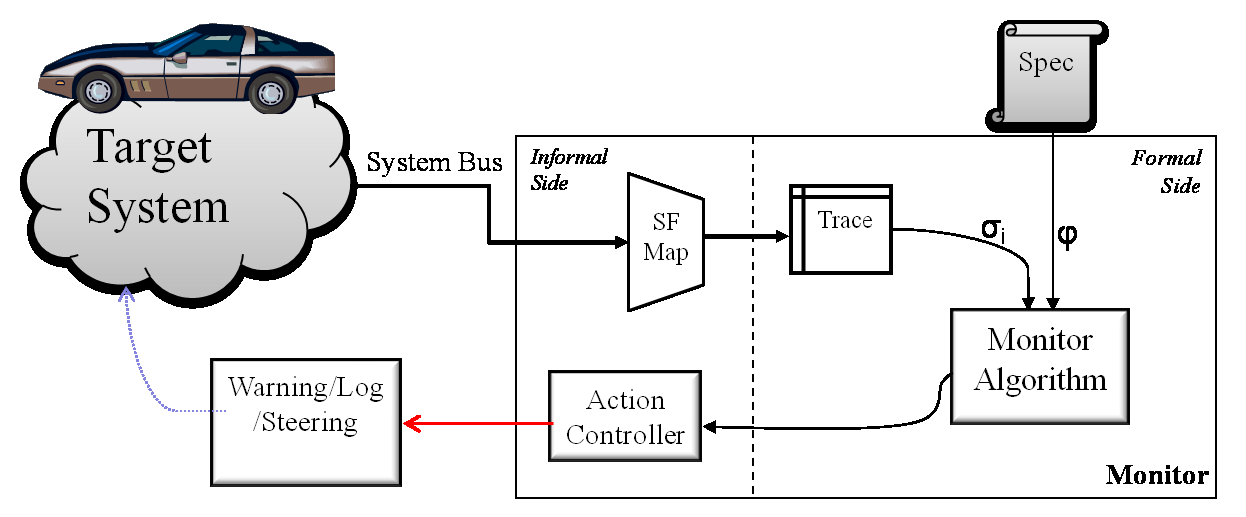
\includegraphics[width=4.5in]{img/mon_arch}
\caption{External monitor architecture outline \label{fig:architecture}}
\end{figure}

This architecture separates the system-independent formal aspects of the monitor from the system-dependent components including the semi-formal interface and system configurations. 
%By utilizing a semi-formal interface, we can separate the formal aspects of the monitor, which are completely independent from the target system, from the more practical pieces: the monitor interfaces and their configurations, which are system dependent. 
This allows us to utilize a core formal monitoring algorithm and framework with any system where an interface map can be used to create a state snapshot. 
Separating the system dependent and system-independent aspects of the monitor also lets the high level system requirements be somewhat abstracted away from the implementation. This means that changes to the target system may only require changes to the interface configuration and not the high level system specification. This is a similar situation to the two-level specifications used in the MaC framework \cite{Kim2004}.

\subsection{System Interface}
Different systems have varying specification needs which can not always be easily met within a formal specification language. In order to provide flexibility to map system state onto the formal specification language (in our case, in propositions) we provide a semi-formal system interface which defines the mapping between the observed system state and the monitored specification. This type of interface is common in monitors for real systems, including MaC's filters \cite{Kim2004} and the AP evaluation filter from \cite{Heffernan2014}.

\subsection{Hybrid Algorithm}
Our eager monitoring algorithm attempts to evaluate specification rules as soon as possible, but this requires checking extra rules


Though early detection of specification violations can be useful, for example to initiate a recovery sooner, performing these eager checks requires more computation.
%
There are situations where eagerly checking a target specification would take too much time to guarantee real-time monitoring correctness. To enable the benefits of eager checking while avoiding the risks of losing real-time correctness, we have implemented a hybrid eager monitoring algorithm which performs non-eager (conservative) checking first and uses any spare time to eagerly check remaining monitor residues.

Under our periodic sampling design, the conservative check is guaranteed to only need to check a single residue for each specification policy in every step (plus updating structures or saving history once per step). 
This conservative check can be done quickly at each period, leaving any extra time until the next check for eager checking. This provides a guarantee that at least the specification is checked within a known delay (i.e., a promptness guarantee) and allows the monitor to eagerly check as much as possible. 
As long as we know that the worst case execution time for message handing, incrementing the structures, and a single residue check is short enough to finish within a monitor period then we are guaranteed at least a conservatively correct and prompt output.

We implemented the hybrid monitoring algorithm in our embedded monitor, which updates the shared monitoring structures and performs a conservative check once every monitoring period, and the uses the idle time between periods to perform eager checking of any remaining unchecked specification properties.
%
Figure \ref{fig:arch:oscope} shows the execution of the embedded monitor instrumented to output the currently executing task to an oscilloscope. This task output was captured using the specification discussed in Section \ref{sec:monspec} plus another 200 time-step \emph{eventually} rule which was never satisfied (so every step the monitor performed all 200 eager checks and could not reduce any remaining formulas. Even with this wasted computation there was still a large portion of idle time -- 23ms of the 25ms loop was spent idle. This shows the eager checking finished reasonably quickly and the monitor could handle much longer formula durations or more complex formulas before the execution time becomes bad enough to not guarantee the monitor finishing all of it's desired eager checking in a single monitoring period. 

\begin{figure}
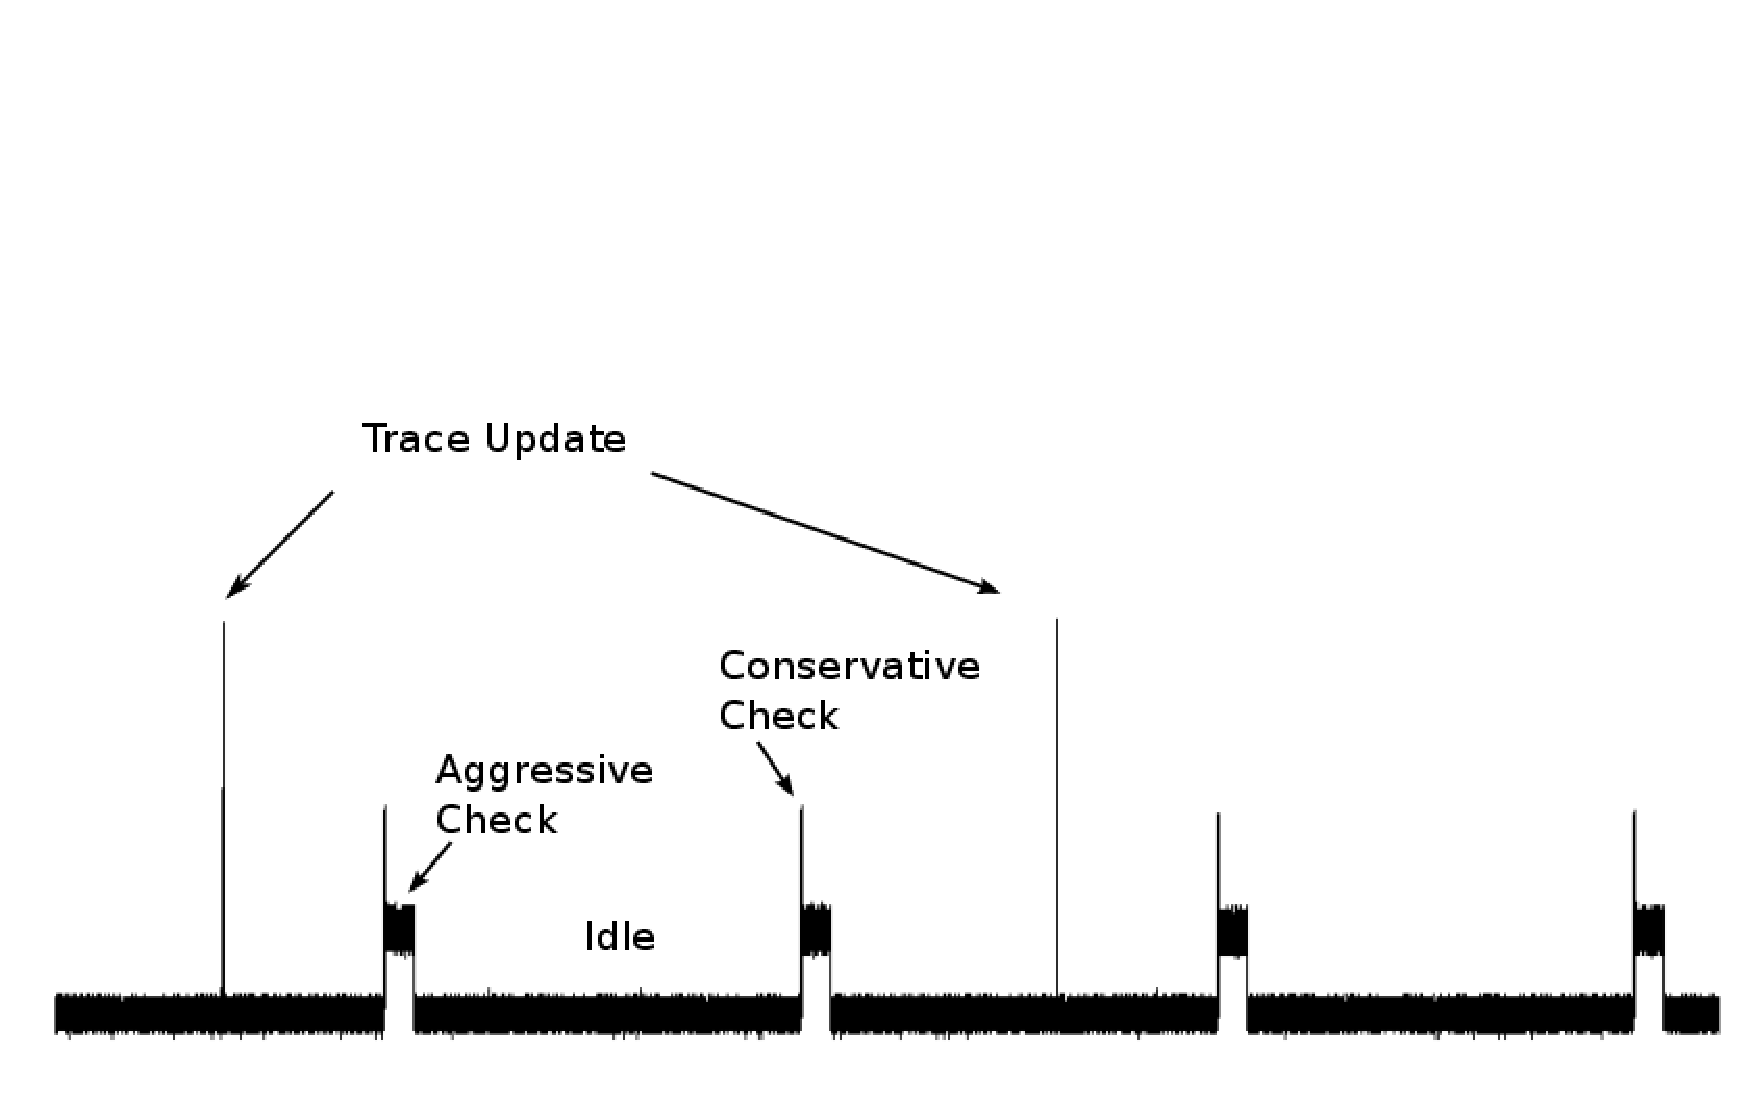
\includegraphics[width=4in]{img/scope_annotated}
\caption{Oscilloscope capture of embedded monitor task execution \label{fig:arch:oscope}}
\end{figure}

%%%%% Algorithm section

\section{Monitoring Algorithm}
%% Why our algorithm... 
%%% MTL due to explicit time restrictions
%%% need real-time finite trace checking

In order to monitor distributed embedded systems we need an algorithm which can continuously check explicit time specifications over finite traces. This has led to our algorithm \monitor which is an iterative monitoring algorithm based on formula reduction (essentially formula-rewriting). 
%
\monitor checks specifications written in a future-bounded metric temporal logic. A large portion of safety specification rules for safety-critical embedded systems require explicit time bounds to ensure timely behavior, so a specification language with explicit time bounds is important. 

To constantly check that the target system is adhering to its specification, we must constantly check the specification against the current system trace. To constantly check the system efficiently, \monitor is an iterative algorithm, performing additional checking as each new trace step arrives.

%The monitoring algorithm is an aggressive, iterative algorithm based on formula reduction (essentially formula-rewriting) and a stored history structure to check whether a given formula satisfies or violates the target trace. 
%It is aggressive in that the algorithm attempts to check future-time temporal formulas as soon as possible rather than wait until an answer is guaranteed to be available (by combining short-circuiting and immediate checking of temporal subformulas).
%This is in contrast to many existing runtime monitoring algorithms which either are restricted to past time logics (in which there is no waiting) or only check properties after their available delay. % some aggressive future time algorithms exist but almost always dynamic programming so can't do windowed bounds
%The algorithm is iterative in that the history structure must be updated at each timestep in the trace in order. 

\subsection{Specification Logic}
In this section, we introduce our safety specification language for embedded systems, which we call \planguage. \planguage is based on \emph{propositional metric temporal logic} (MTL) \cite{}. 
The syntax of our bounded MTL variant \planguage is given below:

%The specification logic is a bounded, propositional metric temporal logic where the target propositions are from a set of atomic propositions provided by the system interface. These propositions are derived from the observable system state and represent system properties, for example, a proposition $speedLT40mph$ could state whether the vehicle speed is less than 40mph.


\(
\begin{array}{ccc}
\policy & ::=  & \true \mid p \mid \neg \policy \mid \policy_1\vee \policy_2\mid
\policy_1\since_{\interval}\policy_2 \mid \policy_1\until_{\interval}\policy_2\mid\yesterday_{\interval}\policy\mid \tomorrow_{\interval}\policy
\end{array}
\)

%Policy formulas are represented by $\psi$. Formulas can include both past time operators ($\since$, $\lastmtl$) and future time operators ($\Until$,$\nextmtl$). Each temporal operator has an associated time interval $\interval$ of the form $[lo,hi]$ where $lo,hi \in \mathbb{N}$ and $lo \leq hi$

We assume we are given a finite set of propositions, denoted by \cP, which can be used to specify safety policies. 
These propositions are generated by the system interface from observable system state.
Each proposition $p\in\cP$ is a formula of \planguage. 
We have logical connectives ($\neg, \vee$) and also have past ($\since, \yesterday$) and future ($\until, \tomorrow$) temporal operators. 
Each temporal operator has an interval (denoted by \interval) associated with it in which the formula is evaluated. 
The interval has the form $[lo, hi]$ where $lo, hi\in\mathbb{N}$ and $lo\leq hi$. 
The interval imposes an additional time interval constraint in which the immediate sub-formula must be true. 
For example, $\policy_1\since_{[lo, hi]}\policy_2$ is true at current time $t$ represents that $\policy_2$ was true in the past within times $t-hi$ to $t-lo$  and from that point on, $\policy_1$ has been true. 
For past temporal operators, we allow the high end point of \interval to be $\infty$. 
However, we require our \policy to be \emph{future bounded}, \ie, the high end-point of \interval associated with all future temporal operators must be finite and bounded. 
This restriction is necessary for the termination of our safety monitoring algorithm, as will be discussed later. 

\Paragraph{Derived Operators. }In our syntax, we present a minimal set of logical connectives and temporal operators. 
Other logical connectives and temporal operators can be derived using the following equivalences. (Logical false) $\false\equiv \neg \true$ . 
(Conjunction) $\policy_1\wedge\policy_2\equiv\neg(\neg\policy_1\vee\neg\policy_2)$. 
(Logical implication) $\policy_1\rightarrow\policy_2\equiv \neg\policy_1\vee\policy_2$. 
(Logical equivalence) $\policy_1\leftrightarrow\policy_2\equiv (\policy_1\rightarrow\policy_2)\wedge(\policy_2\rightarrow\policy_1)$. 
(Past temporal operator ``once'') $\once_{\interval}\policy\equiv (\true\since_{\interval}\policy)$. 
(Past temporal operator ``historically'') $\historically_{\interval}\policy\equiv \neg\once_{\interval}\neg\policy$. 
(Future temporal operator ``eventually'') $\eventually_{\interval}\policy\equiv (\true\until_{\interval}\policy)$. 
(Future temporal operator ``henceforth'') $\henceforth_{\interval}\policy\equiv \neg\eventually_{\interval}\neg\policy$. 


\Paragraph{Semantics. }\planguage formulas are interpreted over time-stamped \emph{traces}. A trace $\sigma$ is a sequence of states, each of which maps all propositions in \cP, to either \true or \false. We denote the $i^{th}$ position of the trace with $\sigma_i$ where $i\in\mathbb{N}$. Moreover, each $\sigma_i$ has an associated time stamp denoted by $\tau_i$ where $\tau_i\in\mathbb{N}$. 
We denote the sequence of time stamps with $\tau$. For all $i, j\in\mathbb{N}$ such that $i < j$, we require $\tau_i < \tau_j$. For a given trace $\sigma$ and time stamp sequence $\tau$, we write $\sigma, \tau, i\models\policy$ to denote that the formula \policy is true with respect to the $i^{th}$ position of $\sigma$ and $\tau$. We define $\sigma, \tau, i\models\policy$  inductively in the following way. 
\begin{itemize}
 \item $\sigma, \tau, i\models\true$
 \item $\sigma, \tau, i\models p$ $\Longleftrightarrow$ $\sigma_i(p) = \true$. 
 \item $\sigma, \tau, i\models\neg\policy$ $\Longleftrightarrow$ $\sigma, \tau, i \not\models\policy$. 
 \item $\sigma, \tau, i\models\policy_1\vee\policy_2$ $\Longleftrightarrow$ $\sigma, \tau, i\models\policy_1$ or $\sigma, \tau, i\models\policy_2$. 
 \item $\sigma, \tau, i\models\policy_1\since_{[lo, hi]}\policy_2$ $\Longleftrightarrow$ there exists a $k\leq i$ such that $lo\leq\tau_i-\tau_k\leq hi$ and $\sigma, \tau, k\models\policy_2$, and for all $j$ such that $k< j\leq i$, $\sigma, \tau, j\models\policy_1$ holds. 
 \item $\sigma, \tau, i\models\policy_1\until_{[lo, hi]}\policy_2$ $\Longleftrightarrow$ there exists a $k\geq i$ such that $lo\leq\tau_k-\tau_i\leq hi$ and $\sigma, \tau, k\models\policy_2$, and for all $j$ such that $i\leq j< k$, $\sigma, \tau, j\models\policy_1$ holds.
 z
 \item $\sigma, \tau, i\models\yesterday_{[lo, hi]}\policy$ $\Longleftrightarrow$ $i > 0$, $lo \leq (\tau_i-\tau_{i-1})\leq hi$, and $\sigma, \tau, i-1\models\policy$.
 \item $\sigma, \tau, i\models\tomorrow_{[lo, hi]}\policy$ $\Longleftrightarrow$ $lo \leq (\tau_{i+1}-\tau_{i})\leq hi$, and $\sigma, \tau, i+1\models\policy$. 
\end{itemize}


Our monitoring algorithm utilizes \emph{residues}, which are partially reduced (\ie, rewritten) policy formulas representing the remaining portion of a formula which could not be fully evaluated given the current trace. A residue $r^j_{\policy}$ is a tagged pair $\rpt{j}{\policyv}{\policy}$ where $j$ is a position in the trace. We use these residues to efficiently hold policy history for future time formulas which cannot be evaluated due to incomplete information.

Policy formulas have a wait delay $\wdelay(\policy)$ which defines an upper bound on the time duration necessary to guarantee complete information to evaluate the formula. Past and present-time formulas have no wait delay, since all trace steps necessary to evaluate them have already been seen by the monitor. Future time formulas have a delay based on their duration. The length $|\policy|$ of a policy $\policy$ is defined as the total number of subformula, (\ie, the number of nodes in the policy AST).

To evaluate \planguage policies, we need to save a limited amount of history state of child policies of temporal subformula within a policy. For example, given the policy $ACCCancelReq \rightarrow \eventually_{\interval} ACCOff \vee (ACCOn \since_{\interval} ACCCancelReq)$, $ACCOff$ is a child policy of the temporal formula $\eventually_{\interval}$ and $ACCOn$ and $ACCCancelReq$ are children of the temporal formula $ACCOn \since_{\interval} ACCCancelReq$. The monitor must store some history of these child policies in order to evaluate the parent policy.
The operation $\tempSub$ identifies all the children of temporal subformula of a policy.
%% might want to do a more abstract example to show recursiveness
%That is, for $\alpha\, \mathcal{U}_{[l,h]}\, \beta$ we need to save the history of $\alpha$ and $\beta$ (and if either of those are also a temporal formula then we need their history as well). 


%% maybe need formula length, storage delay, simplify\dots


\subsection{Monitoring Algorithm}
Our runtime monitoring algorithm \monitor takes as input a specification $\policy$ and monitors a growing trace, building history structures and reporting the specification violations as soon as they are detected. We summarize the relevant algorithm functions below:

\begin{description}
\item[$\monitor{}(\policy)$] is the top-level function. \\
\item[$\reduce(\sigma_i, \tau_i, \histSt{i}, \rpt{i}{\policy}{\policy})$] reduces the given residue based on the current state $(\sigma_i,\tau_i)$ and the history $\histSt{i}$.
\item[$\tempSub(\policy)$] identifies the sub-formulas which require a history structure to evaluate the policy $\policy$.
\item[$\incrS(\histst{i-1}, \histSt{i}, \sigma_i, \tau_i, i)$] updates the history structure $\histst{i-1}$ to step $i$ given the current trace and history state.
\end{description}




\subsubsection{Top-level monitoring algorithm}
The top-level monitoring algorithm \monitor is a sampling-based periodic monitor which uses history structures to store trace state for evaluating temporal subformulas. \emph{History structures} are lists of residues along with past-time markers for evaluating infinite past-time formulas. 
The algorithm checks the given policy $\policy$ periodically at every trace sample step. 
When the policy cannot be decided at a given step (\eg, it requires future state to evaluate), the remaining policy residue is saved in a history structure for evaluation in future steps when the state will be available.
The high level algorithm \monitor is shown in Figure \ref{fig:algorithm}. 

First, all the necessary history structures $\histst[\policyv]{ }$ are identified using $\tempSub(\policy)$ and initialized. 
Once these structures are identified, the monitoring loop begins.
%
In each step, all the history structures are updated with the new trace step. 
This is done in increasing formula size since larger formula can depend on the history of smaller formula (which may be their subformula).
%
Each structure is updated using $\incrS(\histst[\policyv]{i-1},\histSt[\policyv]{i}, \sigma_i, \tau_i, i)$ which adds a residue for the current trace step to the structure and reduces all the contained residues with the new step state. 
Then, the same procedure is performed for the top level policy that is being monitored -- the policy's structure is updated with $\incrS(\histst{i-1},\histSt{i},\sigma_i,\tau_i, i)$.
Once updated, this structure contains the evaluation of the top-level policy. The algorithm reports any identified policy violations (\ie, any $\false$ residues) before continuing to the next trace step.
%
We note that due to the recursive nature of the monitoring algorithm, the top-level policy is treated exactly the same as any temporal subformula would be (which follows from the fact that the top-level policy contains an implicit $\henceforth$). 
The history structures updates for the top-level policy are separated in the algorithm description for clarity only.
The only difference between the top-level policy and temporal subformula is that violations are reported for the top-level policy. 

\begin{figure}
\begin{algorithmic}[1]
%\STATE Recognize formulas for which we build structures
\STATE For all recognized formulas $\policyv \in \tempSub(\policy)$: $\histst[\policy_1]{-1} \leftarrow \emptyset$
\STATE $i \leftarrow 0$
\LOOP
\STATE Obtain next trace step $(\sigma_i, \tau_i)$ 
\FOR{every $\policyv \in \tempSub(\policy)$ in increasing size}
	\STATE $\histst[\policyv]{i} \leftarrow \incrS(\histst[\policyv]{i-1}, \histSt[\policyv]{i}, \sigma_i, \tau_i, i)$
\ENDFOR
\STATE $\histst{i} \leftarrow \incrS(\histst{i-1}, \histSt{i}, \sigma_i, \tau_i, i)$
%\FOR{all $\rp{j}{\bot} \in S^i_{\varphi}$}
\FOR{all $\rp{j}{\false} \in \histst{i}$}
\STATE \texttt{Report violation on $\sigma$ at position $j$}
\ENDFOR
\STATE $i \leftarrow i + 1$
\ENDLOOP
\end{algorithmic}
\caption{\monitor Algorithm}\label{fig:algorithm}
\end{figure}

\subsubsection{Reducing Residues}
\monitor works primarily by reducing policy residues down to truth values. Residues are reduced by the $\reduce(\sigma_i, \tau_i, \histSt{i}, \rpt{j}{\policyv}{\policy})$ function, which uses the current state $\sigma_i,\tau_i$ and the stored history in $\histSt{i}$ to rewrite the policy $\policyv$ to a reduced form, either a truth value or a new policy which will evaluate to the same truth value as the original. For past or present-time formulas, $\reduce()$ is able to return a truth value residue since all the necessary information to decide the policy is available in the history and current state. Future-time policies may be fully-reducable if enough state information is available. If a future-time policy cannot be reduced to a truth value, it is returned as a residue unchanged.

\subsubsection{Incrementing History Structures}
To evaluate past and future-time policies, we must correctly store trace history which can be looked up during a residue reduction. We store the trace history of a policy $\policyv$ in a history structure $\histst[\policyv]{}$. This history structure contains a list of residues for the number of steps required to evaluate the top-level policy. History structures are incremented by the $\incrS(\histst[\policyv]{i-1}, \histSt[\policyv]{i}, \sigma_i, \tau_i, i)$ function. This function takes the previous step's history structure $\histst[\policyv]{i-1}$ and the current state ($\sigma_i,\tau_i$, and the updated smaller history structures $\histSt[policyv]{i}$) and performs two actions:
%\begin{enumerate}
	1) Adds a residue for the current step $i$ to $\histst[policyv]{i-1}$ and
	2) Reduces all residues contained in $\histst[policyv]{i-1}$ with the current state.
%\end{enumerate}
Together, these two actions leave an updated history structure $\histst[policyv]{i}$ which has updated history information for all the required steps.

\subsection{Algorithm Properties}

The following theorem states that \monitor is correct and prompt (returns answers within a bounded delay). The theorem requires that the history structures $\histSt{i}$ be consistent at $i$ with respect to the trace $\sigma,\tau$. This means that the history structures contain the actual history of the trace up to step $i$. The algorithm provides this consistency itself if run iteratively from step $0$.

\begin{theorem}[Correctness and Promptness of \monitor]
For all $i \in \mathbb{N}$, all formula $\varphi$, all time stamp sequences $\tau$ and all traces $\sigma$ it is the case that (1) if $\rp{j}{\false} \in \histst{i}$ then $\sigma, \tau, j \nvDash \policy$ and if $\rp{j}{\true} \in \histst{i}$ then $\sigma, \tau, j \vDash \policy$ (Correctness) and (2) if $\tau_i - \tau_j \geq \wdelay(\policy)$ then if $\sigma, \tau, j \nvDash \policy$ then $\rp{j}{\false} \in \histst{i}$ and if $\sigma, \tau, j \vDash \policy$ then $\rp{j}{\true} \in \histst{i}$ (Promptness)
.
\end{theorem}
\textit{Proof.} By mutual induction on the policy formula $\policy$ and time step $i$. See \cite{TechPaper}

%%%%%%%%%%%%%%%%%%%%%%%%%%% REWRITE LINE %%%%%%%%%%%%%%%%%%%%%
%%%%%%%%%%%%%%%%%%%%%%%%%%% REWRITE LINE %%%%%%%%%%%%%%%%%%%%%

%%% New implementation section 

\section{Monitor Implementation}

%% paragraph 1 -- goals
To evaluate the feasibility of our monitoring algorithm for safety-critical real-time systems we have built a real-time CAN monitor on an ARM Cortex-M4 development board. This allowed us to explore the necessary optimizations and features required to perform real-time checking of realistic safety policies.

%% paragraph 2 -- what we built

%% Embedded restrictions
Software for safety-critical embedded systems typically contains more strict design constraints than less critical software. Two important and common constraints for these systems are avoiding recursion and not using dynamic memory allocations. 
% dynamic memory alloc
Common safety-critical coding guidelines discourage or prohibit dynamic memory allocation to avoid memory leaks.
Because our specification language is bounded, we can avoid dynamic allocation in our \monitor implementation by statically allocating space for the maximum number of entries for our history structures and other temporary data structures.
% recursion
Recursion is also usually prohibited because it can be difficult to guarantee a maximum stack depth when using recursion. Although \monitor utilizes recursion extensively, we can implement \monitor using a traditional iterative traversal of the specification formulas instead.

\subsection{Hybrid Algorithm}
Our eager monitoring algorithm attempts to evaluate specification rules as soon as possible, but this requires checking trace properties which may not be evaluated given the current trace. These unevaluated checks are essentially wasted computation, and in general the majority of the policy evaluations performed by \monitor will be eager checks which may not evaluate.

While early detection of violations can be useful, there are situations where eagerly checking an entire target specification may take longer than available for the monitor to keep up with the system in real-time.
%
To enable the benefits of eager checking while avoiding the risks of losing real-time correctness, we have implemented a hybrid eager monitoring algorithm which performs non-eager (conservative) checking first and uses any spare time to eagerly check the remaining monitor residues.

We can conservatively check \monitor residues by only checking residues which are older than their formula delay, which guarantees that the residue will be reduced.
%
Under our periodic sampling design, the conservative check is guaranteed to only need to check a single residue for each specification policy, plus update the history structures, in every step.
This conservative check can be done quickly at each period, leaving any extra time until the next check for eager checking. This provides a guarantee that at least the specification is checked within a known delay (i.e., a promptness guarantee) and allows the monitor to eagerly check as much as possible. 
As long as we know that the worst case execution time for message handing, incrementing the structures, and a single residue check is short enough to finish within a monitor period then we are guaranteed at least a conservatively correct and prompt output.

We implemented the hybrid monitoring algorithm in our embedded monitor, which updates the shared monitoring structures and performs a conservative check once every monitoring period, and the uses the idle time between periods to perform eager checking of any remaining unchecked specification properties.
%
Figure \ref{fig:arch:oscope} shows the execution of the embedded monitor instrumented to output the currently executing task to an oscilloscope. This task output was captured using the specification discussed in Section \ref{sec:monspec} plus another 200 time-step \emph{eventually} rule which was never satisfied (so every step the monitor performed all 200 eager checks and could not reduce any remaining formulas. Even with this wasted computation there was still a large portion of idle time -- 23ms of the 25ms loop was spent idle. This shows the eager checking finished reasonably quickly and the monitor could handle much longer formula durations or more complex formulas before the execution time becomes bad enough to not guarantee the monitor finishing all of it's desired eager checking in a single monitoring period. 

\begin{figure}
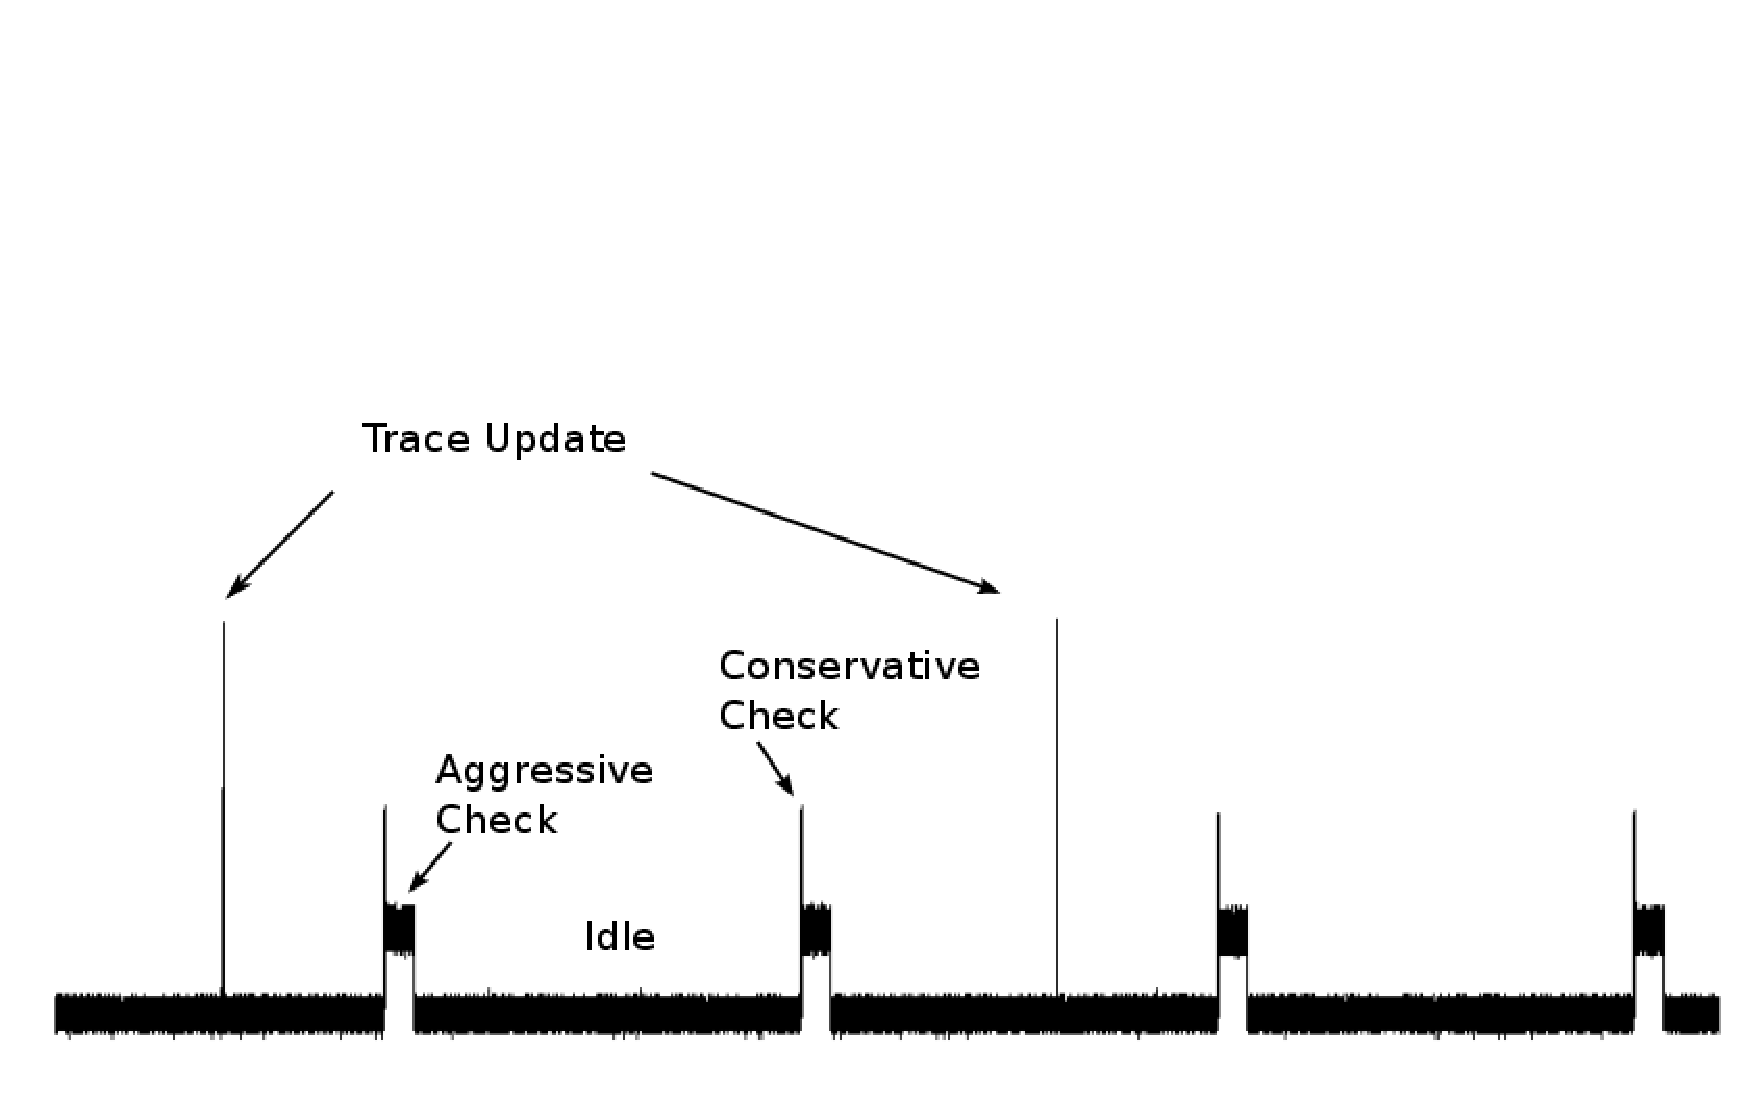
\includegraphics[width=4in]{img/scope_annotated}
\caption{Oscilloscope capture of embedded monitor task execution \label{fig:arch:oscope}}
\end{figure}

%%%%% Case study section


\section{Case Study}

%% paragraph 1 -- experimental environment
This section reports our case study performing real-time monitoring of a CAN network for realistic safety properties. We have implemented the \monitor algorithm on a low cost ARM-Cortex M4 development board which can be used to monitor CAN networks. For this case study we have obtained CAN network logs from a series of robustness tests on an autonomous research vehicle which we have replayed on a test CAN bus for the monitor to check. This setup is shown in Figure \ref{fig:replaySchem}.

\begin{figure}
\centering
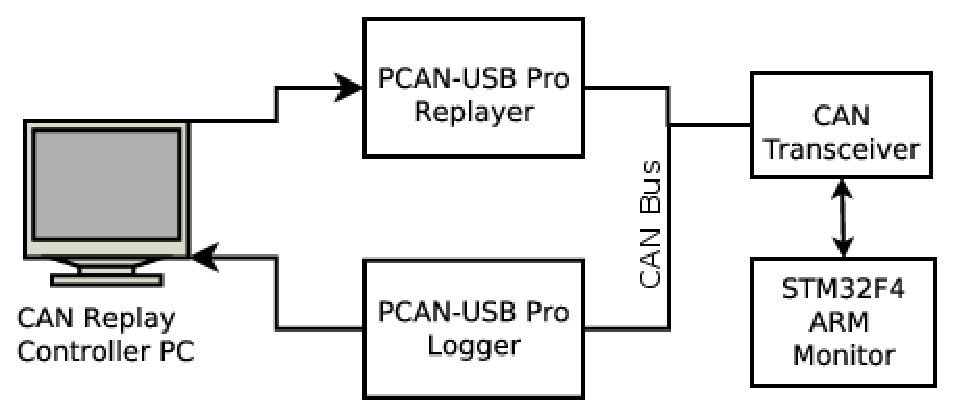
\includegraphics[width=4.5in]{img/replay_arch}
\caption{CAN replay network setup \label{fig:replaySchem}}
\end{figure}

%% paragraph 2 -- experiment goal
We wish to use the CAN monitor to check a realistic set of safety policies over a real network trace. From this, we can see the feasibility of performing external bus monitoring for these types of systems.

%% paragraph 3 -- description of experiment 
%%% some of this is in para1, we should go over: specification, logs, etc
The logs contain both normal operation as well as some operation under network-based robustness testing. During robustness testing, the testing framework can hijack targeted network messages on the bus to inject testing values. % could cite astaa here
A PC was connected to a PCAN-USB Pro \cite{PCAN-USBPro} device which provides a USB interface to two CAN connections. One CAN channel was used as the log replayer, while the other was used as a bus logger for analysis purposes.

%% paragraph 4 -- specification
Requirements documentation for this system was available, so we were able to build a monitoring specification based on actual system requirements.
The specification evaluated in the embedded monitor on the test logs are shown in Table \ref{tab:monspec}. This specification was derived from the system requirements based on the observable system state available in the testing logs. 


Rule \#0 is a heartbeat detection which ensures that the interface component is still running (essentially a watchdog message). Rule \#1 is a second component of this check. The system's heartbeat message contains a single heartbeat status bit which we checked directly in Rule \#0, but the message also has a rolling counter field. We use the system interface to ensure that this counter is correct, and check the system interface's output ($\pred{HeartbeatOk}$) in Rule \#1.
We also checked for illegal state transitions. Rules \#2 through \#5 check both for illegal transition commands and actual illegal state transitions.

\begin{table}
%\begin{tabular}{|p{3in}|l|}
\begin{tabular}{|l|p{4.5in}|}
\hline \multirow{2}{*}{Rule \#} & Informal Rule \\ & BMTL \\
\hline \multirow{2}{*}{0} & A feature heartbeat shall be received every 500ms \\
& $\pred{HeartbeatOn} \rightarrow \lozenge_{[0,500ms]} \pred{HeartBeat}$ \\
\hline \multirow{2}{*}{1} & The interface component heartbeat counter is correct \\
& $\pred{HeartbeatOn} \rightarrow \pred{HeartbeatCounterOk}$ \\
\hline \multirow{2}{*}{2} & The vehicle shall not transition from manual mode to autonomous mode \\
&  $\neg ((\blacksquare_{[1,1]} \pred{IntManualState}) \wedge \pred{IntAutoStat})$\\
\hline \multirow{2}{*}{3} & The vehicle controller shall not command a transition from manual mode to autonomous mode \\
& $\neg ((\blacksquare_{[1,1]} \pred{VehManualModeCmd}) \wedge \pred{VehAutoModeCmd})$\\
\hline \multirow{2}{*}{4} & The vehicle shall not transition from system off mode to autonomous mode \\ 
&  $\neg ((\blacksquare_{[1,1]} \pred{IntSDState}) \wedge \pred{IntAutoStat})$\\
\hline \multirow{2}{*}{5} & The vehicle controller shall not command a transition from system off mode to autonomous mode \\
& $\neg ((\blacksquare_{[1,1]} \pred{VehSDModeCmd}) \wedge \pred{VehAutoModeCmd})$\\
% warn was at 200ms
\hline
\end{tabular}
\caption{Case study monitoring specification \label{tab:monspec}}
\end{table}

\subsection{Monitoring Results}
Monitoring the test logs with the above specification resulted in identifying two real violations as well as some false positive violation detections caused by the testing infrastructure.

% covering all three possible violation types. One was a false positive
Three different types of heartbeat violations were identified after inspecting the monitor results.
% missing hb message
The first is a late heartbeat message. In one of the robustness testing logs the heartbeat message was not sent on time, which is clearly a heartbeat violation. Figure \ref{fig:hb_arrival} shows the heartbeat counter values and the inter-arrival time of the heartbeat messages over time for this violation. We can see here that the heartbeat counter did in fact increment in a valid way, just too slowly. 

\begin{figure}
		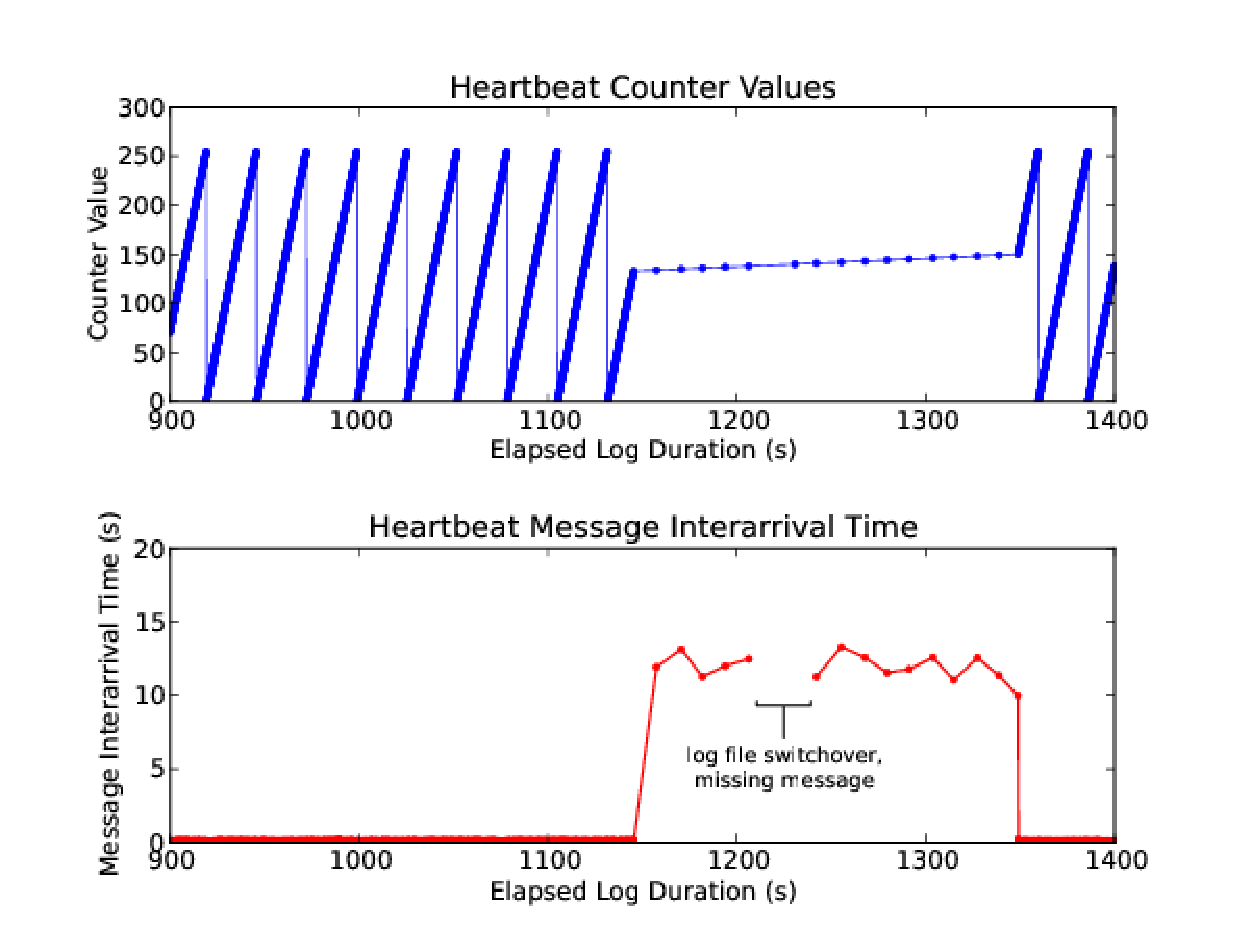
\includegraphics[width=4.5in]{img/hb1}
		\caption{Heartbeat counter values over time}
		\label{fig:hb_arrival}
\end{figure}

% bad status
The second violation is on-time heartbeat status message but the heartbeat status field is 0. 
We do not know from the available documentation whether a bad status in an on-time message with a good counter is valid or not. So without more information we cannot tell whether these violations are false positives or not. This is worthy of further investigation.

% bad counter
The last type of violation is a bad counter. 
We have defined a good counter as one which increments by one every message up to its maximum (255 in this case) before wrapping back to zero.
Every consecutive heartbeat status message must have an incremented heartbeat counter or a violation will be triggered. Figure \ref{fig:hb_badcounter} shows the counter value history for one of the traces with a heartbeat violation caused by a bad counter value.
%
%@EDIT describe robustness testing, define these false positives like the talk?
Further inspection of this violation showed that the bad counter values were sent by the testing framework rather than the actual system. In this case, the network traffic the monitor is seeing is not real system state but actually it is messages being injected by the testing framework. This is not a real violation (since the violating state is not the actual system state), and so we consider this a false positive violation.


\begin{figure}
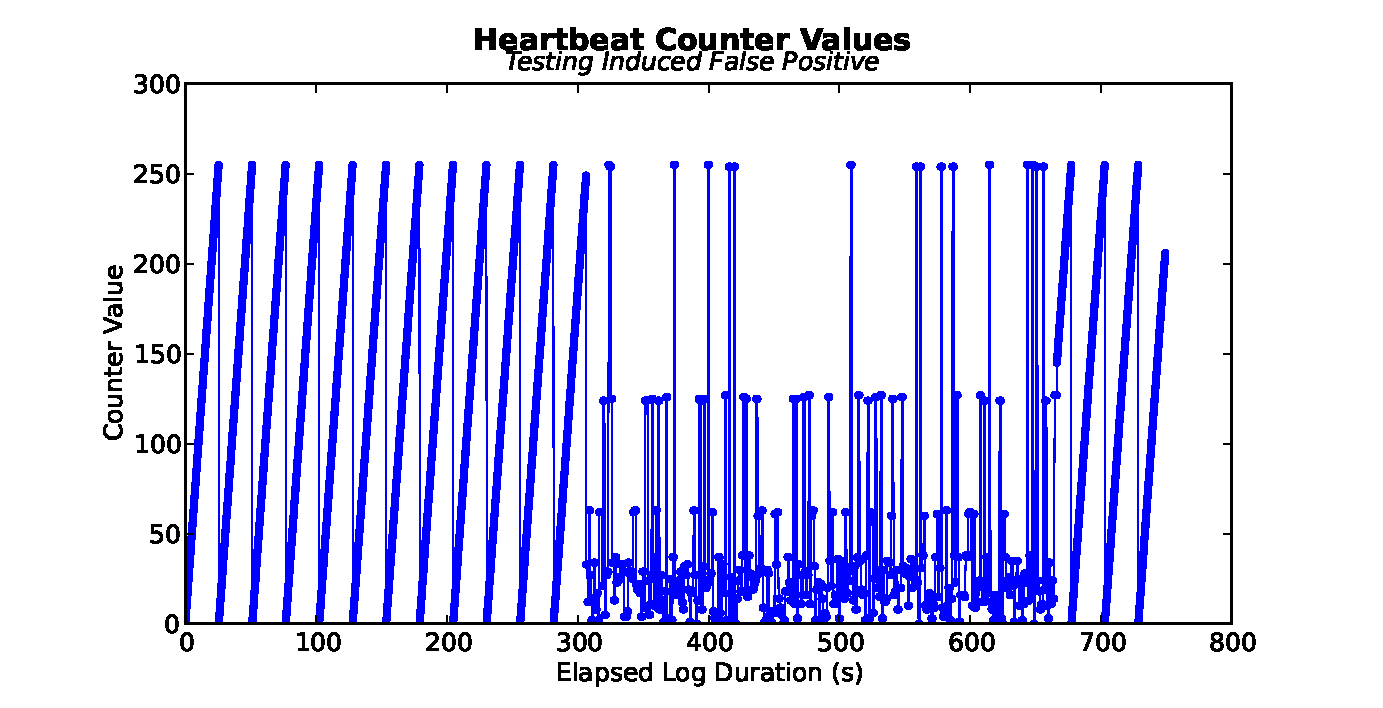
\includegraphics[width=4.5in]{img/hb2}
\caption{Bad heartbeat counter values \label{fig:hb_badcounter}}
\end{figure}

The monitor also reported violations of the legal transition rules, but these, similar to the heartbeat counter violation, also turned out to be false positives triggered by message injections by the robustness testing harness. Since the monitor checks network state, if we perform testing that directly affects the values seen on the network (such as injection/interception of network messages) we may detect violations which are created by the testing framework rather than the system. 
Information about the test configurations can be used to filter out these types of false positives which arise from test-controlled state.
This type of filtering can be automated if the test information can be input to the monitor, either directly on the network (e.g., adding a message value to injected messages) or through a side-channel (i.e., building a testing-aware monitor).

%%%% Conclusion section

\section{Conclusion}
We have developed a runtime monitoring approach for ARV system. 
%We have developed an online, real-time monitoring approach that targets an autonomous research vehicle, describing our experience. 
Rather than instrumenting the target system, we passively monitor the system, generating the system trace from the observed network state.
We have developed an efficient runtime monitoring algorithm, \monitor, that eagerly checks for violations of properties written in our future-bounded propositional MTL. 
We have shown the efficiency of \monitor by implementing it and evaluating it against logs obtained from system testing of the ARV. 
\monitor was able to detect violations of several safety requirements in real-time.



%\def\IEEEbibitemsep{0pt plus .5pt}
\bibliographystyle{splncs03}
% argument is your BibTeX string definitions and bibliography database(s)
%\tiny
\bibliography{./rv2015_bibtex}
%\end{small}
%\bibliography{./rv2015_bibtex}

\end{document}
